\section{Main Program}
\label{main-program}

The general idea is to build an UI with three main divisions: Home (with device
selection), midi selection and signal-to-MIDI connections, Plot (with the signal
visualization) and Options (with the algorithm tuning options, as well as virtual
MIDI creation).\\
When a device is selected it's signals will go through a simple process, as in \autoref{signals-flow-diagram}.
\begin{figure}[htb]
	\caption{Signals Flow Diagram}
  \label{signals-flow-diagram}
	\begin{center}
    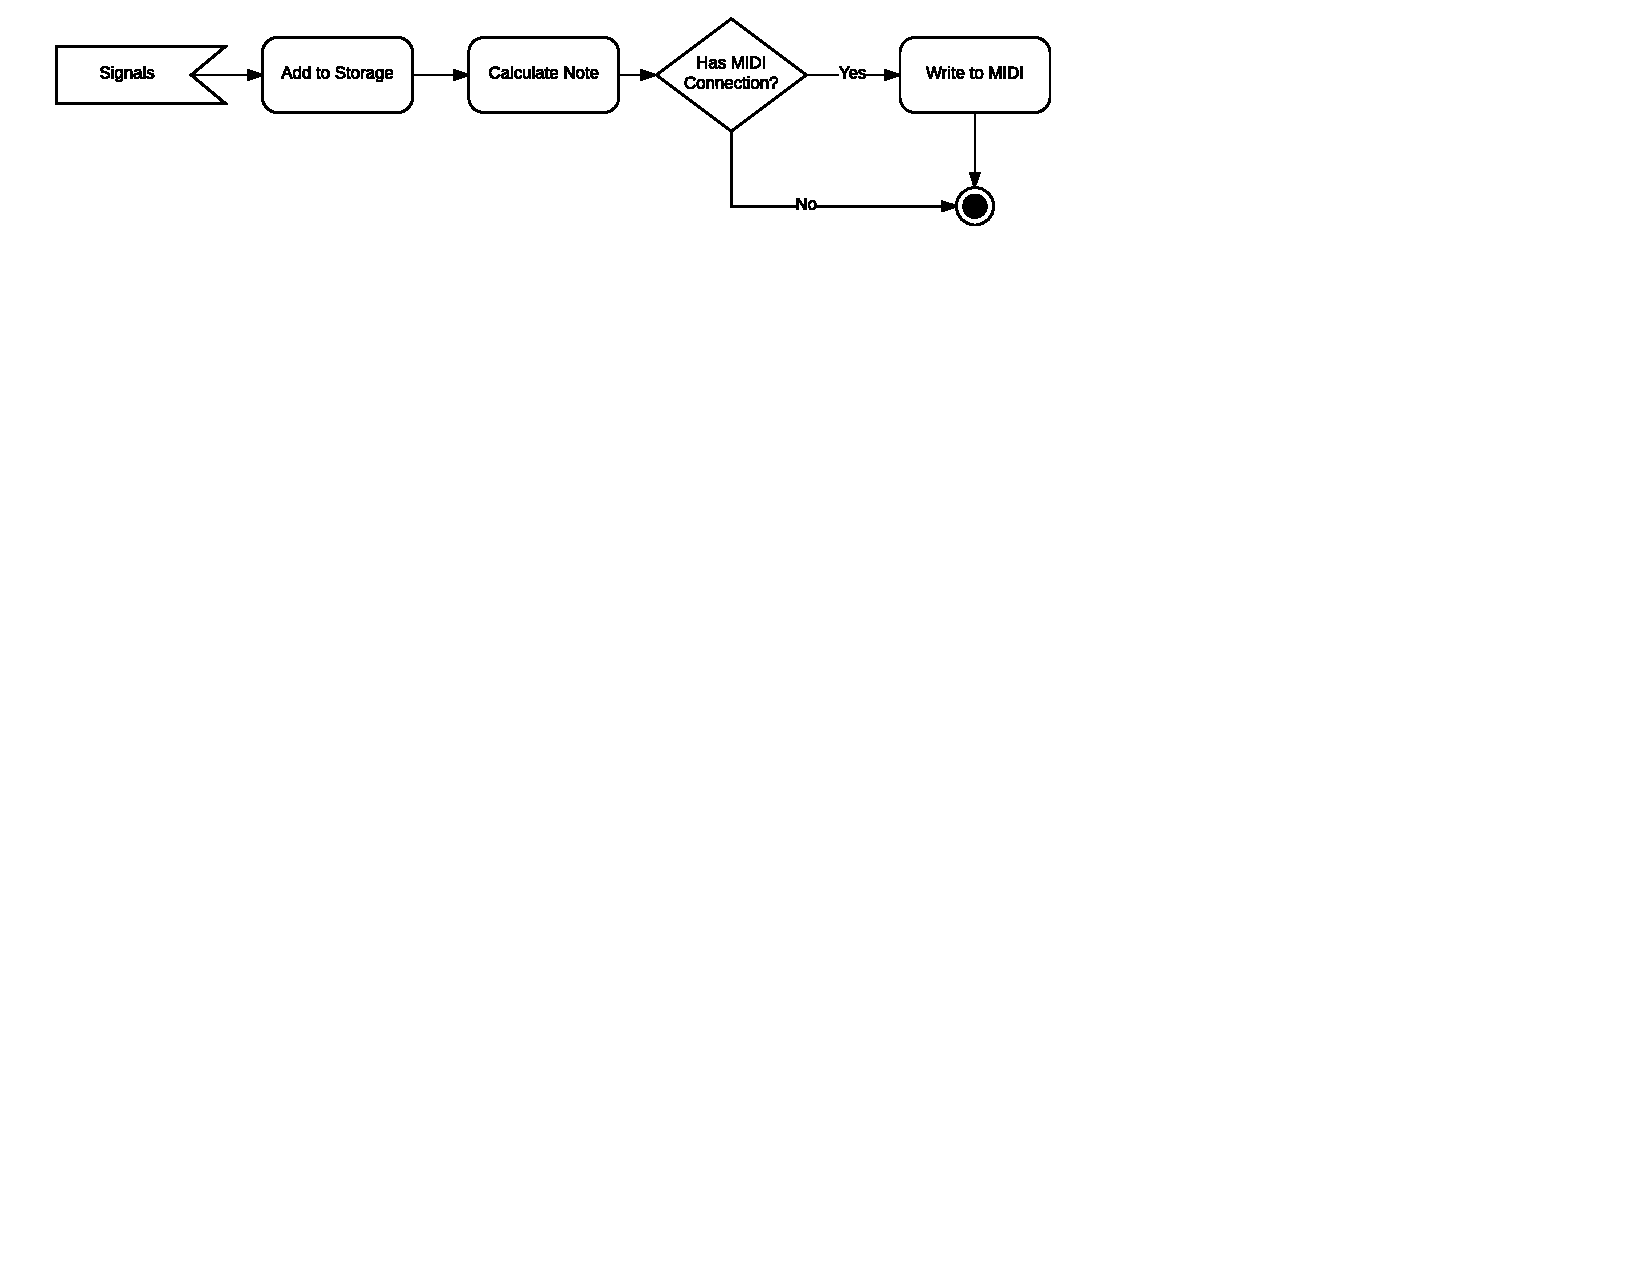
\includegraphics[scale=0.9]{images/signals-flow-diagram}
	\end{center}
  \legend{Source: authors}
\end{figure}

\subsection{GUI}

\subsubsection{Home}
The home page has three horizontally divided sections: Device and signals, MIDI selection
and list, and  finally connections, as in \autoref{home-page}. \\
The first is used to open the device (there can be only one used at a time). When it
is open a list of signals will be displayed (six of them, named as each guitar note).
Each signal can be selected so it can be connected to a MIDI device.\\
The second is to open any given number of existing MIDI devices, which will be listed
bellow (can be also closed). The listed devices can also be selected, but only one at a time. \\
The final section is used to establish the connections, given the selected signals
and MIDI, the connections are showed in the box bellow and can be deleted.
\begin{figure}[htb]
	\caption{Home Page}
  \label{home-page}
	\begin{center}
    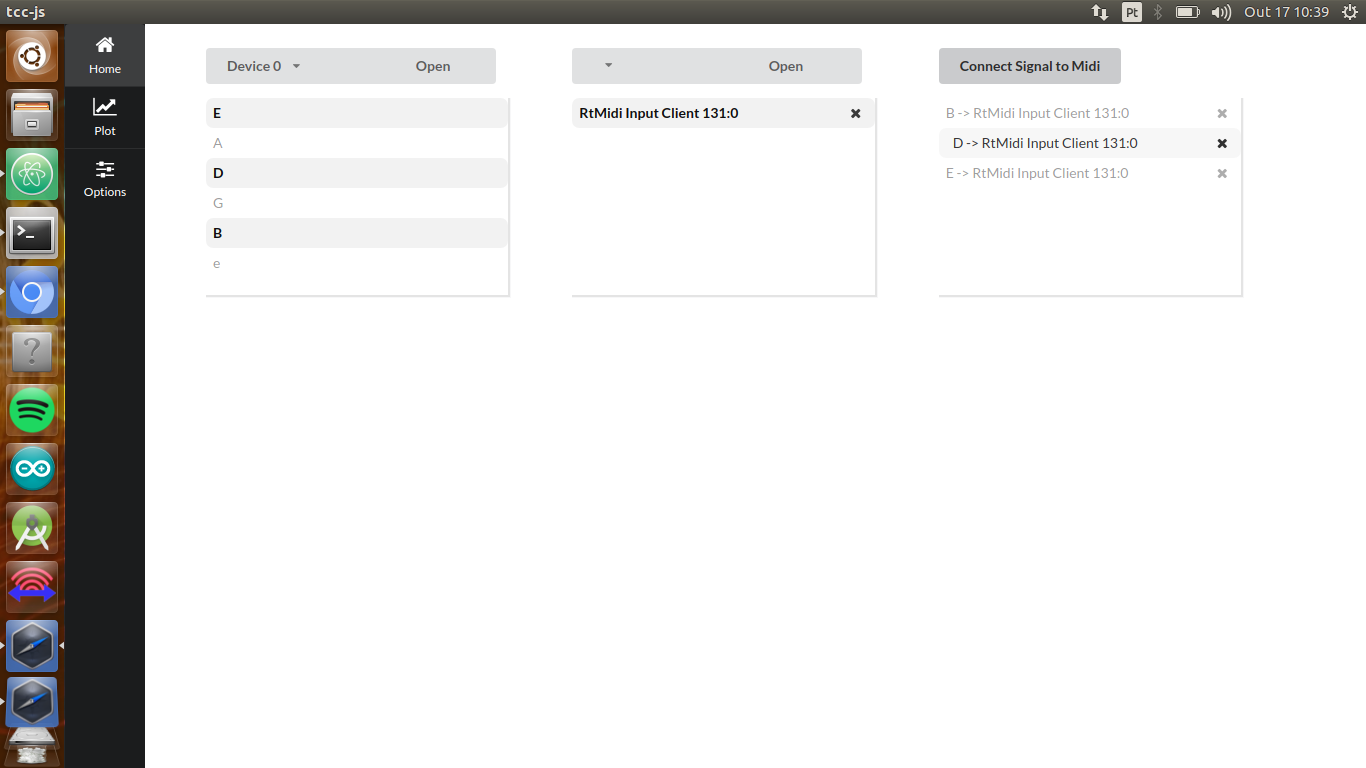
\includegraphics[width=0.7\paperwidth]{images/snapshots/home}
	\end{center}
  \legend{Source: authors}
\end{figure}

\subsubsection{Plot}
The Plot page is a simply a react-plotter \cite{react-plotter} component with a few
visual controls, being: a dropdown to select which signal is being displayed,
a checkbox to enable trigger, a slider to control the time
range and another slider to control the trigger value. The full page is as in \autoref{plot-page}.
It was chosen to show only one plot at a time so it's size is bigger, easier to see.
This also makes the program a little more performant.
\begin{figure}[htb]
	\caption{Plot Page}
  \label{plot-page}
	\begin{center}
    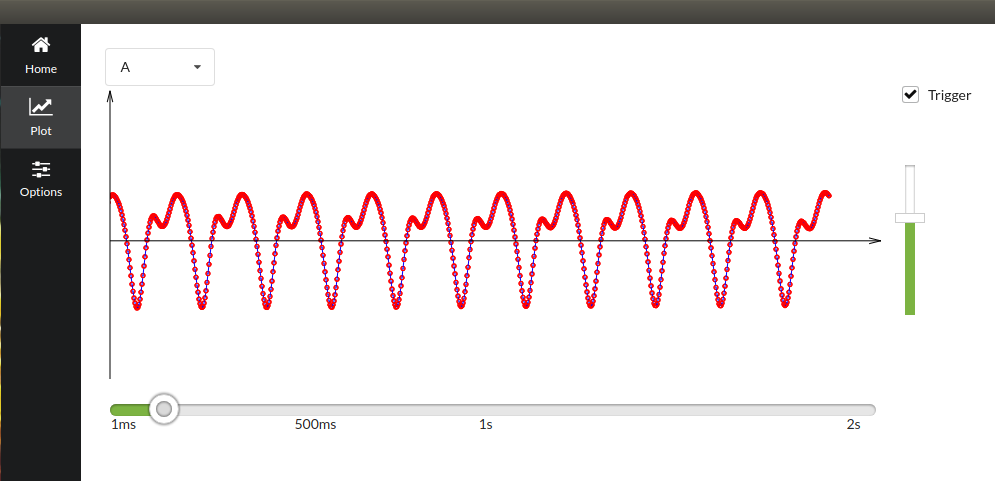
\includegraphics[width=0.7\paperwidth]{images/snapshots/plot-trigger-A}
	\end{center}
  \legend{Source: authors}
\end{figure}

\subsubsection{Options Page}
The options page is simply an UI to control the used algorithm (from \autoref{pitch-detection})
and it's parameters. For both Linux and macOS it's also possible to create virtual
MIDI devices, from which our program can write and a synthesizer can read. For Windows
this is still possible, but using a hacky solution (since Windows does not give any
official API for this) - the easiest option being LoopBe1 \cite{LoopBe1}. The
page can be seen at \autoref{options-page}.
\begin{figure}[htb]
	\caption{Options Page}
	\label{options-page}
	\begin{center}
		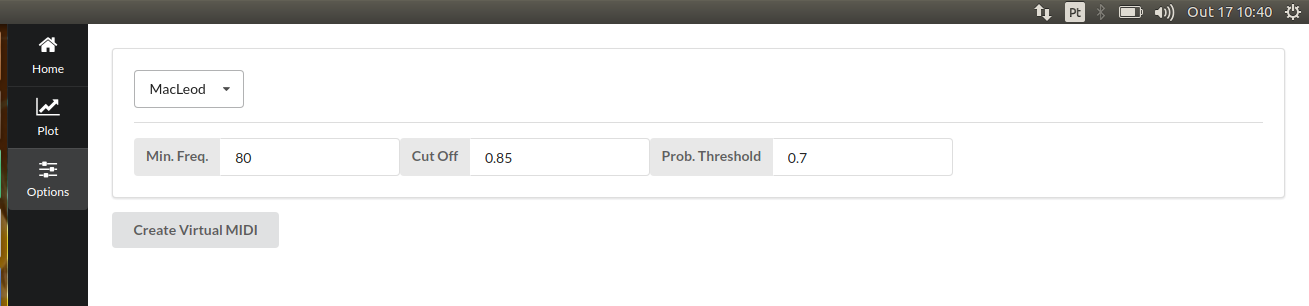
\includegraphics[width=0.7\paperwidth]{images/snapshots/options}
	\end{center}
	\legend{Source: authors}
\end{figure}

\subsection{Implementation}

\subsubsection{Resources}
At first let's take a look at our resorces:
\begin{itemlist}
	\item USB device: only one can be connected
	\item MIDI devices: a list of them can be used at any time
	\item Signals: fixed for the only connected device
\end{itemlist}
It's easy to see they are all global, so they can be represented as static classes.
But JavaScript has good functional programming capabilities, which are very
suitable for global resources. JavaScript imported modules are also scoped, by default,
this means it works like a C++ namespace, keeping our static resources separated in
a nice way. Taking these mentions in account three modules were built for resource
easy access, being MIDI, USB and signal processing.

\subsubsection{Entry Point}
The entry point for our project is both a declarator and connector. It allocates
all needed structures (or calls the module that does it), the most significant one
being the Redux store \cite{Redux} - store being a short for storage, which is
where all of our application visible state is held. \\
The entry point also connects all callbacks and logic in a declarative way. In
this single file all of the program's internal functionalities are declared,
so much that if you read it you should also understand the entire program.

\subsubsection{Reducers}
Redux stored data is not defined by a set a properties, like typical OOP applications,
instead it uses a more functional programming paradigm. The storage is defined by transfer
functions, each of them describing actions that can modify the current state by
returning a new one. Each of these functions, called reducer, receive two parameters -
the current state and the action to be processed - and should return the new state
for the action (or the current one if there are no changes). \\
Our program has nine reducers, but five of them share the same transfer function,
as in \autoref{reducers-table}.
\begin{table}[htb]
  \ABNTEXreducedfont
  \caption[Reducers]{Reducers}
  \label{reducers-table}
  \centering
  \begin{tabular}{c|c|c|c}
    \textbf{Name} & \textbf{Data Type} & \textbf{Actions} & \textbf{Used for} \\
		\hline \hline
		device & string & set, remove & current selected device \\
		\hline
		devices & string[ ] & add, remove & list of devices \\
		\hline
		signals & string[ ] & set, clear & list of signals \\
		\hline
		signalsData & object[ ]: {name: number[ ]} & set, clear & list of signals data (name and values) \\
		\hline
		object & object: any & set, clear, remove & Plot Page options \\
																					& & & General options \\
																					& & & MIDI devices \\
																					& & & Signal to MIDI connections \\

  \end{tabular}
  \legend{Source: authors}
\end{table}

\subsubsection{Note Calculation}
To calculate the note a few steps are shown in \autoref{note-detection-diagram}.
The amplitude calculation is a simple absolute avareage removing the mean. The
pitch within range is a function that limits each string frequency to
being close to it's know possible values, as in \autoref{pitch-range-table}.
\begin{figure}[htb]
	\caption{Note Detection Diagram}
	\label{note-detection-diagram}
	\begin{center}
		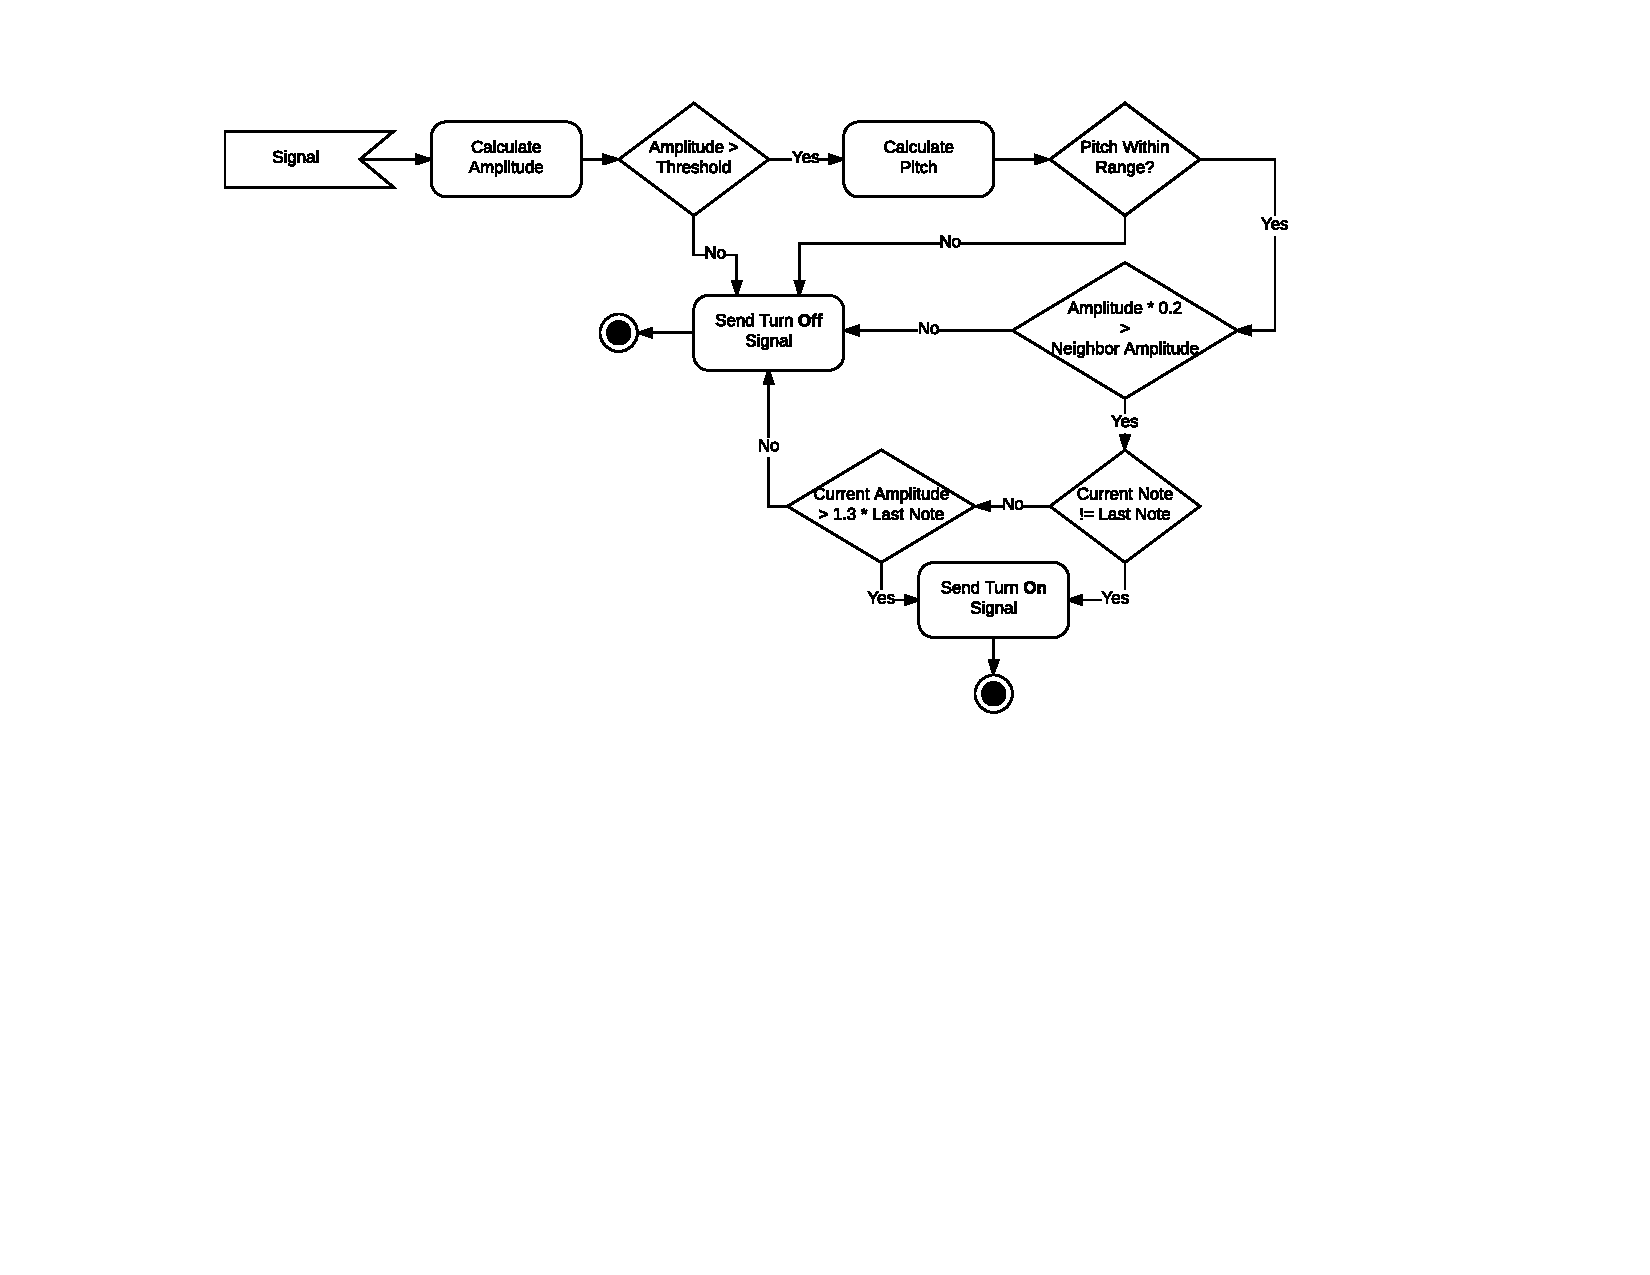
\includegraphics[width=0.7\paperwidth]{images/note-detection-flow-diagram}
	\end{center}
	\legend{Source: authors}
\end{figure}

\begin{table}[htb]
  \ABNTEXreducedfont
  \caption[Pitch Range]{Pitch Range}
  \label{pitch-range-table}
  \centering
  \begin{tabular}{c|c|c}
    \textbf{String} & \textbf{Min. Freq.[Hz]} & \textbf{Max. Freq.[Hz]} \\
		\hline \hline
		E & 70 & 265 \\
		\hline
		A & 95 & 350 \\
		\hline
		D & 130 & 470 \\
		\hline
		G & 170 & 625 \\
		\hline
		B & 215 & 785 \\
		\hline
		e & 290 & 1050 \\
  \end{tabular}
  \legend{Source: authors}
\end{table}

\subsubsection{Tests}
This is for now a prototype of a real world project, so it has a limited amount
of tests. The tests fall into one of two categories: unity or timing. Unity tests
are made for the signal processing relating modules and also for every reducer,
these are all automated and sum up to a total of 31 tests over 9 modules. \\
The timing tests were used to check if each separated functionality that may
cause processing issues can run in real-time. There are timing tests for: signal
average value calculation, signal window buffering, raw data conversion,
pitch detection and USB polling.

\subsubsection{Repository}
Again, all code is available at GitHub \cite{guitar-digitizer}.
